\begin{frame}[t]
  \slideheader{05. THE SOLUTION}{Find the passage, not just the song.}

  % Dominant Visual: Centerpiece Interface Screenshot with Caption
  {\centering
  \begin{tcolorbox}[standardcard, width=8.2cm, top=1.5pt, bottom=2.5pt, left=1.5pt, right=1.5pt]
    \centering
    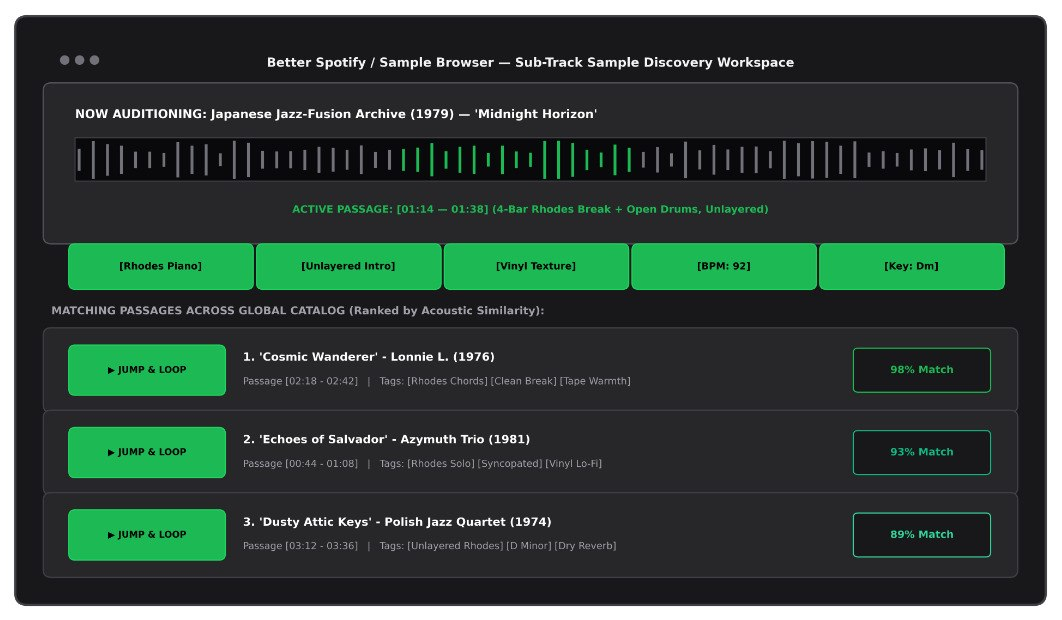
\includegraphics[width=\linewidth, height=3.8cm, keepaspectratio]{images/sample_browser_mockup.png}\par\vspace{1mm}
    {\tiny\textcolor{textdim}{Concept mockup (illustrative; match scores are not from a working algorithm)}}
  \end{tcolorbox}\par}

  \vspace{1.5mm}

  % Three Concise Capability Labels
  \begin{columns}[onlytextwidth, c]
    \begin{column}{0.315\textwidth}
      \begin{tcolorbox}[innercard, top=2.5pt, bottom=2.5pt]
        \centering
        {\scriptsize\bfseries\textcolor{accentemerald}{1. Acoustic Filters}}\par\vspace{0.2mm}
        {\tiny\textcolor{textmuted}{Instrument, texture, timbre}}
      \end{tcolorbox}
    \end{column}

    \begin{column}{0.315\textwidth}
      \begin{tcolorbox}[innercard, top=2.5pt, bottom=2.5pt]
        \centering
        {\scriptsize\bfseries\textcolor{accentemerald}{2. Passage Results}}\par\vspace{0.2mm}
        {\tiny\textcolor{textmuted}{Timestamped section candidates}}
      \end{tcolorbox}
    \end{column}

    \begin{column}{0.315\textwidth}
      \begin{tcolorbox}[innercard, top=2.5pt, bottom=2.5pt]
        \centering
        {\scriptsize\bfseries\textcolor{accentemerald}{3. Direct Cue + Loop}}\par\vspace{0.2mm}
        {\tiny\textcolor{textmuted}{Instant playhead jump (\texttt{seekTo})}}
      \end{tcolorbox}
    \end{column}
  \end{columns}
\end{frame}
